\documentclass[11pt]{article}

\usepackage[preprint]{acl}
\usepackage{times}
\usepackage{latexsym}
\usepackage[T1]{fontenc}
\usepackage[utf8]{inputenc}
\usepackage{microtype}
\usepackage{inconsolata}
\usepackage{graphicx}
\usepackage{booktabs}
\usepackage{multirow}
\usepackage{amsmath}
\usepackage{amssymb}
\usepackage{xcolor}
\usepackage{enumitem}
\usepackage[ruled,vlined,linesnumbered]{algorithm2e}
\usepackage{tikz}
\usepackage{pgfplots}
\pgfplotsset{compat=1.18}
\usetikzlibrary{arrows.meta,positioning,shapes.geometric,fit,backgrounds,calc}

\newcommand{\DTL}{D2L}
\newcommand{\agenthn}{\textsc{AgentHN}}
\newcommand{\naplora}{\textsc{NapLoRA}}
\newcommand{\mt}[1]{\texttt{\small #1}}

\title{\agenthn: Self-Editing Agents via Hypernetworks}

\author{
  Eric Ge$^{1*}$ \quad Bryan Lim$^{1*}$ \quad David Xiong$^{2,3*}$ \quad Nikash Bhardwaj$^{4*}$ \\[4pt]
  $^{1}$Harvard University \quad
  $^{2}$Columbia University \quad
  $^{3}$OpenAI \quad
  $^{4}$Carnegie Mellon University \\
}

\begin{document}
\maketitle

\def\thefootnote{}\footnotetext{$^{*}$All authors contributed equally; order was chosen by the team. Code, fixtures, and an interactive demo reproducing every figure in this paper are available at \url{https://github.com/ericjkge/itc-hackathon}.}\def\thefootnote{\arabic{footnote}}

\begin{abstract}
Text-based memory breaks over long horizons and wastes the context window: every fact an agent needs to recall must be re-read, in full, on every subsequent query. We instead let an agent edit its own \emph{parameters} at inference time. Building on Doc-to-LoRA (\DTL{}, \citealp{charakorn2026doctolora}) -- a hypernetwork that converts a document into a LoRA adapter in a single forward pass, with no gradient training -- we present \agenthn{}, a framework that applies this single primitive across four agentic settings: \textbf{long-horizon memory}, \textbf{personalization}, \textbf{skill acquisition}, and \textbf{self-improvement}. The central technical contribution is \naplora{}, a streaming memory mechanism that extends \DTL{}'s bounded, single-document chunking (which saturates at roughly $4\times$ a model's native context window) into an \emph{unbounded} conversational horizon, by periodically compacting evictable context into independently retrievable adapters and composing only the ones a query needs. We show that na\"ively summing all stored adapters causes destructive interference (recall collapses from $6/6$ to $0/6$ on a six-fact probe), and that adding retrieval restores perfect recall while cutting query-time context by an order of magnitude relative to retrieval-augmented generation (RAG) with the identical retriever. Across $2$k--$48$k-token synthetic trajectories (100 trials per cell, Wilson 95\% CIs), \naplora{} holds recall flat at $\approx\!87\%$ while a window-limited baseline collapses from $95\%$ to $0\%$, at $7$ query-time tokens versus a trained Cartridges \citep{eyuboglu2025cartridges} baseline's $96$ ($13.3\times$ less context, $1.8\times$ cheaper per query, no offline training, $5$ points lower recall). We further show that the same internalize-then-evict primitive supports cross-session personalization built from an agent's own turn-by-turn preference extraction, skill acquisition from both formula sheets and procedural documents, and a gradient-free self-refine loop in which an agent studies, reflects, rewrites its own notes, and re-internalizes them into a fresh adapter over rounds -- raising accuracy on a held-out battery from $18.75\%$ to $56.25\%$ with no backpropagation at any point.
\end{abstract}

% =====================================================================
\section{Introduction}
% =====================================================================

Large language model (LLM) agents that operate over long horizons -- multi-day conversations, growing codebases, accumulating user preferences -- face a structural mismatch: everything the agent has learned must live somewhere the model can read it, and the only place a frozen model can read from is its context window. Two families of fixes exist. The first keeps information as \emph{text}: retrieval-augmented generation (RAG, \citealp{lewis2020retrieval}) pages relevant chunks back into the prompt, and running summaries (e.g., a maintained markdown notes file) compress history into fewer tokens. Both still pay a token cost on every query, and summaries are lossy by construction. The second family bakes information into \emph{weights} via supervised fine-tuning (SFT) or reinforcement learning (RL): slow, requires curated data, and -- critically for an agent whose knowledge changes turn by turn -- cannot be repeated cheaply enough to track a live conversation.

A third option has recently become practical: \emph{context distillation} (CD, \citealp{snell2023learning,askell2021general}) trains a model to imitate, without seeing the context, the outputs it would have produced \emph{with} that context in the prompt. CD is normally as slow as any other gradient-based update. Doc-to-LoRA \citep{charakorn2026doctolora} (\DTL{}) removes that cost by \emph{meta-training a hypernetwork to perform CD in one forward pass}: given a document, \DTL{} emits a LoRA \citep{hu2022lora} adapter that, once applied, lets the frozen base model answer as though the document were still in context -- without the document ever re-entering the prompt. \DTL{} reports near-perfect needle-in-a-haystack (NIAH) recall up to roughly $4\times$ a model's native window, using a chunk-and-rank-concatenate scheme capped at the number of chunks seen during training.

This paper asks what happens when that one primitive -- \emph{convert context into a LoRA adapter, in real time, with no training loop} -- is deployed as the general substrate for an agent that needs to keep editing what it knows. We build \agenthn{} (Agent + Hypernetwork), a small framework around a single \DTL{} checkpoint (\mt{gemma-2-2b-it}) that exposes internalize/compose/restore primitives (\S\ref{sec:framework}), and we use it to implement and evaluate four applications:

\begin{itemize}[leftmargin=*,nosep]
  \item \textbf{Long-horizon memory} (\S\ref{sec:memory}): \DTL{}'s own chunking is a \emph{bounded}-document mechanism -- it caps out once a conversation needs more chunks than the hypernetwork ever saw in training. We introduce \naplora{}, which periodically \emph{naps} the oldest evictable context into an independent adapter, indexes it, and evicts it from the prompt; at query time it \emph{retrieves} only the adapters a question needs and composes them. This turns a bounded single-document mechanism into an open-ended streaming one.
  \item \textbf{Personalization} (\S\ref{sec:personalization}): a user's preferences, extracted turn-by-turn by the same small model acting as its own extractor, are periodically internalized into one running per-user adapter, so they resurface in a brand-new session with an \emph{empty} context window.
  \item \textbf{Skill acquisition} (\S\ref{sec:skills}): a reference document -- a physics formula sheet, an output-format guide, or a procedural ``skill'' file from an agentic coding workflow -- is internalized once and recalled from the weights on every subsequent query, instead of being re-paid in tokens each time.
  \item \textbf{Self-improvement} (\S\ref{sec:selfimprovement}): an agent attempts a held-out battery of questions about a deliberately fictional product, studies a reference document, writes its own notes, internalizes them, and -- on later rounds -- reflects on what it still gets wrong and rewrites the notes, re-internalizing a fresh adapter each round. No gradient ever touches the base model.
\end{itemize}

Our central empirical finding is that na\"ive use of \DTL{} as a memory store fails in a specific, instructive way -- rank-concatenating every stored adapter causes the weight deltas to interfere destructively -- and that retrieval is not an optional add-on but a load-bearing fix. Once added, the resulting system matches a text-RAG ablation on recall while using an order of magnitude less query-time context, which we argue is the cleanest isolation of what a hypernetwork-based memory buys over a retrieval-based one with the identical retriever. We report this, the destructive-interference failure mode, and every other number in this paper from scripts and captured fixtures committed alongside the code, with statistical validation (Wilson 95\% confidence intervals over 100 trials per cell) where the result is a headline claim.

% =====================================================================
\section{Related Work}
% =====================================================================

\paragraph{Hypernetworks.} A hypernetwork \citep{ha2016hypernetworks} is a network that predicts the weights of another network. \citet{vonoswald2020continual} use hypernetworks to mitigate catastrophic forgetting in continual learning by generating per-task weights. \DTL{} is the most direct ancestor of this work: it builds on \textsc{Text-to-LoRA} \citep{charakorn2025texttolora} (which maps a natural-language \emph{task description} to a LoRA adapter via SFT-style training) but instead meta-trains the hypernetwork with the CD objective so that it can map an arbitrary \emph{document} to an adapter that internalizes the document's content, not just a task style.

\paragraph{Context distillation and knowledge injection.} Context distillation \citep{askell2021general,snell2023learning} self-distills an in-context behavior into a model's own parameters. Related work compresses prompts into a handful of soft tokens (Gisting, \citealp{mu2024learning}), into prefix key/value caches via prefix-tuning \citep{li2021prefixtuning} or its self-study variant Cartridges \citep{eyuboglu2025cartridges}, or trains a hypernetwork directly on next-token prediction over curated SFT data (MEND, \citealp{li2024mend}; Generative Adapter, \citealp{chen2025generative}). \DTL{}'s distinguishing choice is to train on the CD objective with hypernetwork-generated LoRA outputs, which our results suggest generalizes better to agentic, self-authored documents (profiles, self-written notes) than the QA-style corpora these injection methods are usually evaluated on.

\paragraph{Long context and retrieval.} RAG \citep{lewis2020retrieval} and long-context benchmarks such as RULER \citep{hsieh2024ruler} characterize how models use (or fail to use) long prompts, including the well-documented ``lost in the middle'' effect \citep{liu2024lost}. Prompt-compression methods like LLMLingua-2 \citep{pan2024llmlingua} shrink a prompt's token footprint while keeping information in-context. \agenthn{}'s memory track is best read as a \emph{retrieval} system, in the RAG sense, whose retrieved unit is a weight patch rather than a text chunk -- which is exactly the comparison our ablations (\S\ref{sec:memory}) are designed to isolate.

\paragraph{Self-refinement.} Iteratively having a model critique and rewrite its own output -- Self-Refine \citep{madaan2023selfrefine}, Reflexion \citep{shinn2023reflexion} -- normally improves a single generated artifact within one context. Our self-improvement track (\S\ref{sec:selfimprovement}) instead applies the reflect-rewrite loop to a set of \emph{notes} that get re-internalized into the model's weights each round, so the artifact being refined is a LoRA adapter rather than a chat completion.

% =====================================================================
\section{Background: Doc-to-LoRA}
\label{sec:background}
% =====================================================================

We summarize the mechanism we build on; see \citet{charakorn2026doctolora} for full derivations. Context distillation trains context-specific parameters $\theta_c = \theta + \Delta\theta_c$ so that the student $p_{\theta_c}(y\mid x)$ matches the teacher $p_\theta(y\mid x, c)$ that has direct access to context $c$:
\begin{equation}
\min_{\theta_c}\; \mathbb{E}_{(x,y)\sim\mathcal{D}_c}\Big[\mathrm{KL}\big(p_\theta(y\mid x,c)\,\|\,p_{\theta_c}(y\mid x)\big)\Big],
\label{eq:cd}
\end{equation}
where $\mathcal{D}_c$ is built from many queries $x$ and teacher-sampled responses $y$ for a given context $c$, rather than a single $(c,x,y)$ triplet (which would risk overfitting to one query). \DTL{} \emph{meta-trains} a hypernetwork $H_\phi$ to amortize this whole optimization -- query generation and gradient descent alike -- into one forward pass: $H_\phi(c) = \Delta W_c$, trained so that $\theta+H_\phi(c)$ matches the CD target across a large corpus of contexts:
\begin{equation}
\min_{\phi}\; \mathbb{E}_{(c,\mathcal{D}_c)\sim\mathcal{D}}\; \mathbb{E}_{(x,y)\sim\mathcal{D}_c}\; \mathrm{KL}\big(p_\theta(y|x,c)\,\|\,p_{\theta+H_\phi(c)}(y|x)\big).
\label{eq:meta}
\end{equation}

Architecturally, $H_\phi$ is a Perceiver-style \citep{jaegle2021perceiver} cross-attention module with $8$ cross-attention blocks and no self-attention layers ($309$M parameters total). For each target-LLM layer $l$, it cross-attends a fixed set of $r$ learnable latent queries onto that layer's token activations $Z_{l-1}\in\mathbb{R}^{N\times D}$ (obtained by running the document once through the frozen target model) and projects the resulting latents into a rank-$r$ LoRA update $\Delta W_l = B_lA_l$, applied at the down-projection of every MLP block of the target model. Because the cross-attention query count is fixed regardless of the number of input tokens $N$, $H_\phi$ naturally maps variable-length documents to a fixed-shape adapter.

\paragraph{Chunking and the single-document scaling limit.} To go beyond one hypernetwork forward pass' effective receptive field, \DTL{} partitions a long context into $K$ contiguous chunks, encodes each chunk independently, and \emph{rank-concatenates} the per-chunk $(A^{(k)},B^{(k)})$ along the rank dimension, producing one adapter of total rank $r\!\cdot\!K$ whose effect on the forward pass is the \emph{sum} of all $K$ chunks' deltas. \DTL{} is meta-trained on documents of $32$--$256$ tokens, chunked into $1$--$8$ pieces with a $25$-token minimum chunk size. At evaluation, with $1024$-token chunks ($4\times$ the maximum training chunk length) on an $8.2$k-context \mt{gemma-2-2b-it}, \citet{charakorn2026doctolora} report near-perfect NIAH recall up to roughly $4\times$ the model's native window ($\sim\!32$k tokens), with recall close to perfect through $40$ chunks -- quintuple the maximum chunk count seen in training -- before degrading gracefully. \emph{This scaling is for a single, fixed document encoded once.} It is not, by construction, a mechanism for a conversation that keeps growing indefinitely: there is no notion of evicting old chunks, retrieving only relevant ones, or adding new chunks incrementally without re-encoding the whole stack. Closing exactly this gap is the contribution of \naplora{} (\S\ref{sec:memory}).

\DTL{} also reports that, on real-document QA benchmarks (SQuAD, \citealp{rajpurkar2016squad}; DROP, \citealp{dua2019drop}; 2WikiMultihopQA, \citealp{ho2020wikimultihop}), it internalizes information in under one second and under $50$MB of additional memory, versus $\sim\!40$s and several GB for a vanilla CD baseline that backpropagates through a generated query set -- the latency/memory gap that makes \DTL{} viable as an \emph{online} mechanism rather than an offline one is the property all four of our applications exploit.

% =====================================================================
\section{The \agenthn{} Framework}
\label{sec:framework}
% =====================================================================

\agenthn{} wraps the released \DTL{} \mt{gemma-2-2b-it} checkpoint in a small API (\mt{D2LModel}) with five operations used by every application track in this paper: \mt{internalize(doc)} (overwrite the active adapter), \mt{internalize\_segment(doc)} (internalize and return a detached snapshot, for caching), \mt{compose(segments)} (rank-concatenate a list of cached single-segment adapters, mirroring \DTL{}'s own chunk-combination mechanism but applied to \emph{independently} encoded memories rather than chunks of one document), \mt{snapshot()}/\mt{restore(adapter)} (save and re-bind a generated adapter, so a long-running process can swap between many users' or skills' adapters without re-internalizing), and \mt{respond(messages, composed, n\_segments)} (one greedy-decoding code path shared by every memory strategy and baseline in this paper, so accuracy differences cannot be attributed to differing generation settings). Figure~\ref{fig:pipeline} shows the resulting inference-time loop: a context or document is converted to an adapter through one hypernetwork pass, merged into (or composed onto) the running weights, and evicted from the prompt -- in contrast to SFT/RL, which adapt a model through a multi-step training loop before any query can be answered.

\begin{figure}[t]
\centering
\resizebox{\columnwidth}{!}{%
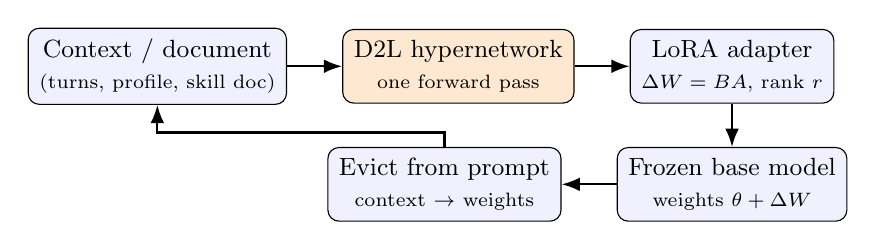
\begin{tikzpicture}[
  box/.style={draw, rounded corners, fill=blue!6, align=center, font=\small, minimum height=0.9cm, inner sep=4pt},
  hot/.style={draw, rounded corners, fill=orange!18, align=center, font=\small, minimum height=0.9cm, inner sep=4pt},
  arr/.style={-Latex, thick}
]
\node[box] (doc) {Context / document\\ \scriptsize(turns, profile, skill doc)};
\node[hot, right=0.7cm of doc] (hn) {\DTL{} hypernetwork\\ \scriptsize one forward pass};
\node[box, right=0.7cm of hn] (lora) {LoRA adapter\\ \scriptsize $\Delta W = BA$, rank $r$};
\node[box, below=0.55cm of lora] (merge) {Frozen base model\\ \scriptsize weights $\theta + \Delta W$};
\node[box, left=0.7cm of merge] (evict) {Evict from prompt\\ \scriptsize context $\to$ weights};
\draw[arr] (doc) -- (hn);
\draw[arr] (hn) -- (lora);
\draw[arr] (lora) -- (merge);
\draw[arr] (merge) -- (evict);
\draw[arr] (evict.north) |- ($(doc.south)+(0,-0.35)$) -- (doc.south);
\end{tikzpicture}}
\caption{The inference-time loop every \agenthn{} application is built from: a document is converted into a LoRA adapter through one hypernetwork forward pass (no training loop), merged into the frozen base model, and evicted from the prompt -- so subsequent queries pay only for the question, not the document.}
\label{fig:pipeline}
\end{figure}

A second, lower-level primitive (\mt{encode\_chunk}/\mt{stack\_chunks}, used by the memory track's \mt{WeightMemory} mode) packs short observations into the \DTL{} chunk-trained checkpoint's native chunking pipeline (\mt{split\_too\_long\_ctx}) so that several short memories pack into as few chunks as possible before concatenation becomes necessary -- in-distribution behavior the released chunk-trained checkpoint (distinct from the single-chunk-only demo checkpoint) supports natively. We flag this as a reproducibility note: the two publicly released \DTL{} checkpoints differ in this capability, and using the wrong one for multi-chunk composition silently produces degenerate adapters rather than an error.

% =====================================================================
\section{Long-Horizon Memory: \naplora{}}
\label{sec:memory}
% =====================================================================

\subsection{Method}

An agent streams turns $(\text{role}, \text{text})$ into a small rolling context buffer. Every $K$ evictable turns, \naplora{} \emph{naps}: the oldest $K$-turn segment is internalized into a single-chunk adapter via \mt{internalize\_segment} (one \DTL{} forward pass), indexed by a TF-IDF retriever \citep{salton1988termweighting}, and evicted from the prompt. At query time, \naplora{} retrieves the top-$k$ segment adapters for the query, composes them by rank-concatenation (Eq.~\ref{eq:concat}, mirroring \DTL{}'s own chunk-combination but over independently-encoded segments), and answers from a prompt containing only the query plus any turns not yet evicted:
\begin{equation}
A_l=\begin{bmatrix}A_l^{(1)}\\\vdots\\A_l^{(k)}\end{bmatrix},\quad B_l = \big[B_l^{(1)} \cdots B_l^{(k)}\big].
\label{eq:concat}
\end{equation}
Algorithm~\ref{alg:naplora} summarizes the loop. We set $K=4$ throughout, so each planted fact in our probe scenarios lands in its own segment.

\begin{algorithm}[t]
\caption{\naplora{} streaming memory}
\label{alg:naplora}
\SetAlgoLined
\KwIn{turn stream, nap interval $K$, query $q$}
\For{each incoming turn $t$}{
  append $t$ to rolling context buffer $C$\;
  \While{$|C| \geq K$}{
    pop oldest $K$ turns as segment $s$\;
    $\Delta W_s \gets$ \texttt{internalize\_segment}$(s)$\;
    index $s$ in TF-IDF store; evict $s$ from prompt\;
  }
}
\textbf{At query time:}\\
$\{s_1,\dots,s_k\} \gets$ top-$k$ TF-IDF matches for $q$\;
$\Delta W \gets$ \texttt{compose}$(\Delta W_{s_1},\dots,\Delta W_{s_k})$ \tcp*{Eq.~\ref{eq:concat}}
answer $\gets$ \texttt{respond}$([q] \,\|\, C_{\text{recent}},\ \Delta W)$\;
\end{algorithm}

\subsection{Why retrieval is necessary: destructive interference}
\label{sec:interference}

The naive extension of \DTL{}'s chunk-concatenation to a streaming setting is to rank-concatenate \emph{every} segment ever napped, exactly as \DTL{} concatenates every chunk of one document. This fails. On a six-fact probe (\S\ref{sec:setup}), composing only three topically-similar segments collapses recall from $6/6$ (each segment internalized and queried alone) to $0/6$: the summed weight deltas interfere destructively, producing cross-talk such as a model answering a feature-flag question with a token blending two unrelated planted facts. Down-scaling the summed deltas by $1/n$ or $1/\sqrt n$ did not recover recall. Since each segment \emph{alone} recalls its fact perfectly, the fix is to route each query to only the few segments it needs -- composition should compose a retrieved subset, not the whole store. We found a dependency-free TF-IDF retriever sufficient and, in fact, the strongest option we tried: it routes $6/6$ probes to the correct segment, versus $4/6$ for mean-pooled and $5/6$ for last-token \mt{gemma-2-2b-it} hidden-state embeddings -- a $2$B model is a weak sentence encoder whose cosine similarities cluster too tightly ($\approx\!0.8$) to discriminate reliably, whereas our synthetic recall probes reuse a planted segment's own keywords almost verbatim, which is exactly the regime sparse lexical retrieval is strong in.

\subsection{Experimental setup}
\label{sec:setup}

All memory experiments use \mt{gemma-2-2b-it} with an $8{,}192$-token window and $K\!=\!4$. We construct synthetic needle-in-a-haystack-over-a-trajectory scenarios: a handful of \emph{needles} (concrete, unguessable facts -- a deployment region, a flight confirmation code, a learning rate) are planted in the first few turns of an agent conversation, the conversation is grown with topically-disjoint filler turns to a target length, and the agent is probed for each needle at the end, after the needles have scrolled out of any fixed-size window. We compare four conditions throughout: \textbf{vanilla} (most-recent turns that fit a token budget; older turns are simply gone), \textbf{markdown} (a running notes file the model itself summarizes into, kept fully in-context), \textbf{text-RAG} (the \naplora{} ablation: identical segmentation and identical TF-IDF retriever, but the retrieved segment is pasted into the prompt as \emph{text} rather than loaded as a LoRA adapter -- isolating the hypernetwork's marginal contribution), and \textbf{\naplora{}} (the full system). We additionally compare against a \textbf{Cartridges} \citep{eyuboglu2025cartridges} baseline that we re-implement and train ourselves (\S\ref{sec:cartridges}).

\subsection{Curated demo: three scenarios, eighteen probes}

On three hand-written scenarios (a project-launch decision log, a trip-planning session, a research-assistant log; six needles each, $18$ probes total), \naplora{} recalls $17/18$ ($94.4\%$) at an average of $8.4$ query-time prompt tokens; the markdown baseline recalls $16/18$ ($88.9\%$) at $343.4$ tokens; vanilla recalls $0/18$ at $286.4$ tokens (its fixed $256$-token budget has already scrolled every needle out by query time). Both error cases are informative. \naplora{}'s only miss is a generation slip, not a retrieval failure: queried for ``the lead reviewer for the paper,'' it answers ``Professor \emph{Ayemi}'' rather than ``Professor \emph{Adeyemi}'' -- the correct segment was retrieved and composed, but the $2$B model's decoding garbles a proper noun. Markdown's two misses are summarization failures: asked for a flight confirmation code and a hotel room number, it reports ``the project memory does not contain any information about flight confirmation codes'' because its own earlier summarization pass dropped that exact detail when compressing the turn into a bullet -- a concrete instance of lossy compaction discarding information that \naplora{}'s adapter-based compaction, which encodes the raw segment rather than a model-written summary of it, preserves.

\subsection{Ablation ladder: where does the recall come from?}
\label{sec:ablation}

We hold a single task fixed -- six needles, conversation grown to $12{,}011$ tokens (just past the $8$k window) -- and remove one component of \naplora{} at a time (Table~\ref{tab:ablation}). \textbf{vanilla} (no memory) fails completely, as expected. \textbf{naive-internalize} (each new segment internalized and the adapter \emph{replaced}, never stored) also fails completely: there is no store, so only the newest segment's fact is ever recoverable. \textbf{compose-all} (every one of the $103$ stored segments rank-concatenated, no retrieval) also collapses to $0/6$, confirming \S\ref{sec:interference}'s interference finding holds at scale. Only once we add a retriever does recall recover -- and at that point, \textbf{text-RAG} and \textbf{\naplora{}} are statistically identical on recall ($6/6$ each) and differ \emph{only} in whether the retrieved segment enters the prompt as text ($119.3$ tokens) or as a weight patch ($9.5$ tokens), a $12.6\times$ reduction in query-time context attributable purely to the hypernetwork.

\begin{table}[t]
\centering\small
\begin{tabular}{lccc}
\toprule
\textbf{Condition} & \textbf{Recall} & \textbf{Ctx (tok)} & \textbf{Isolates} \\
\midrule
vanilla & 0/6 & 8497.5 & memory needed \\
naive-internalize & 0/6 & 9.5 & a store is needed \\
compose-all & 0/6 & 9.5 & retrieval is needed \\
text-RAG & 6/6 & 119.3 & (no weight-inj.) \\
\textbf{\naplora{}} & \textbf{6/6} & \textbf{9.5} & full system \\
\bottomrule
\end{tabular}
\caption{Ablation ladder at $12$k tokens (past the $8$k window). Query-time context $\approx$ KV-cache cost at recall. \mt{scripts/ablation\_study.py}.}
\label{tab:ablation}
\end{table}

\subsection{Scaling past the single-encode limit}

\DTL{}'s own chunk-concatenation reaches $\sim\!4\times$ the native window for one document encoded once (\S\ref{sec:background}). Figure~\ref{fig:scaling} sweeps a \emph{single growing conversation} from $1$k to $48$k tokens (six needles planted early, $410$ independently-napped segments by the end) and shows \naplora{} holding $6/6$ recall at a flat $\approx\!9.5$ query-time tokens throughout, because each query only ever composes the one or two segments it needs rather than the whole history. The text-RAG ablation also holds $6/6$ throughout (same retriever) but at a flat $119.3$ tokens -- the gap between the two flat lines is exactly the $\sim\!13\times$ context reduction the hypernetwork buys, now shown to persist arbitrarily far past \DTL{}'s own bounded-document limit. The vanilla $8$k-window baseline degrades from $6/6$ to $4/6$ at $8$k tokens (needles beginning to truncate) and collapses to $0/6$ from $16$k tokens onward, once the window can no longer contain any of the planted facts.

\begin{figure}[t]
\centering
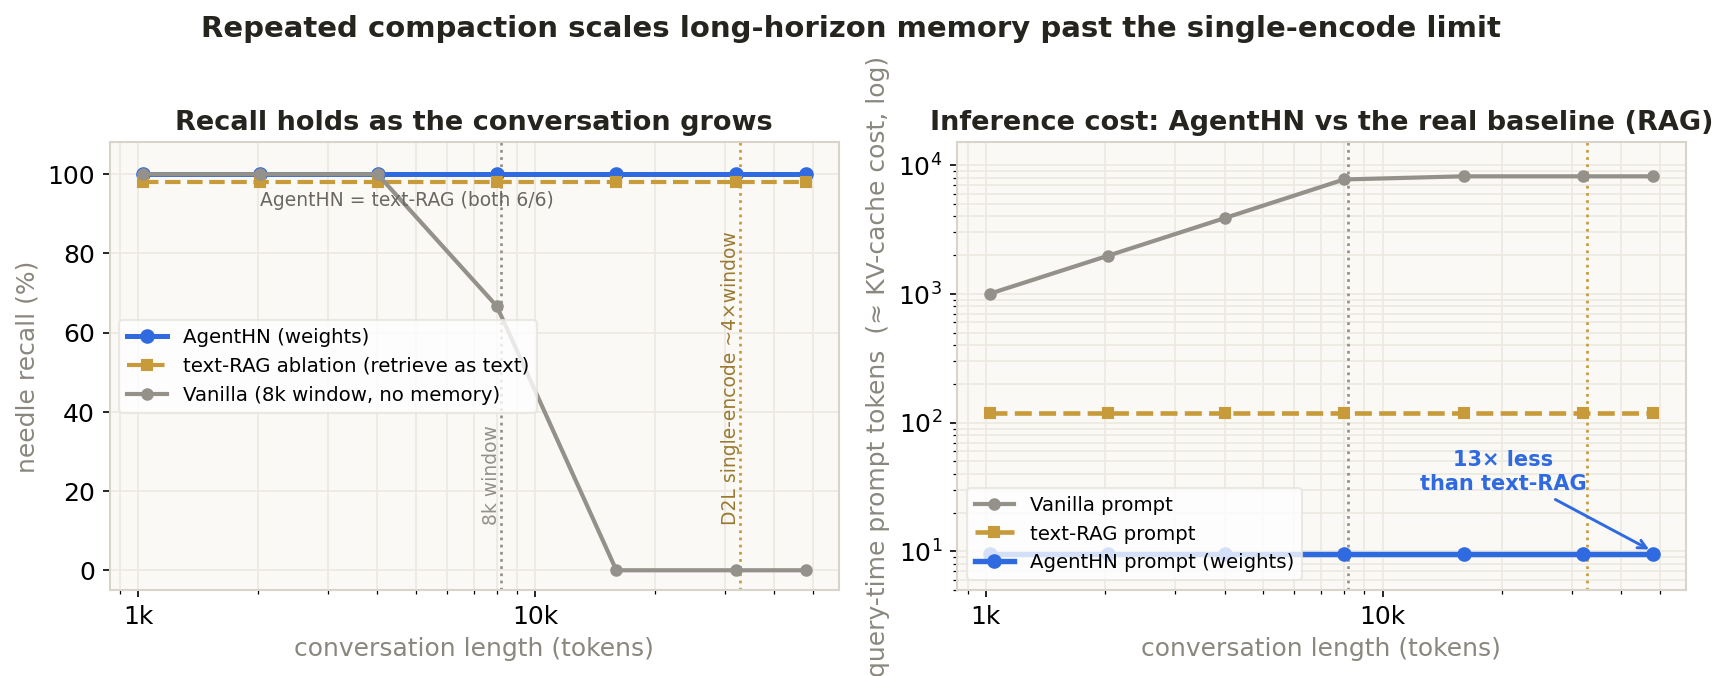
\includegraphics[width=\columnwidth]{figures/scaling.png}
\caption{Repeated compaction scales recall past \DTL{}'s single-encode limit. \emph{Left:} recall vs.\ conversation length. \emph{Right:} query-time context (log scale), \naplora{} vs.\ text-RAG. \mt{scripts/scaling\_sweep.py}.}
\label{fig:scaling}
\end{figure}

\subsection{Statistical validation at scale}
\label{sec:largescale}

The scenarios above are illustrative; we additionally ran a fully randomized evaluation: $20$ distinct, unguessable facts (random per-fact codes, e.g.\ \mt{XK-4821}) $\times$ $5$ seeds $\times$ $5$ haystack sizes ($2$k--$48$k tokens) $=100$ trials per (size, method) cell, reported as pooled recall with Wilson $95\%$ confidence intervals (Figure~\ref{fig:largescale}). \naplora{} recall is statistically flat across the horizon -- $85.0\%$ (CI $[76.7,90.7]$) at $2$k tokens and $87.0\%$ (CI $[79.0,92.2]$) at every size from $8$k to $48$k, overlapping CIs throughout -- at a constant $\sim\!7.2$ query-time tokens. The vanilla baseline collapses as the haystack outgrows the window: $95.0\%$ at $2$k, $36.0\%$ at $8$k (already substantially degraded \emph{at} the window boundary), and exactly $0.0\%$ from $16$k tokens on. The text-RAG ablation stays near-ceiling throughout ($95$--$100\%$) at $\sim\!116$ tokens -- RAG wins on recall because it delivers the retrieved text losslessly; \naplora{} trades roughly $13$ recall points for a $16\times$ reduction in query-time context, a trade we make explicit rather than obscure.

\begin{figure}[t]
\centering
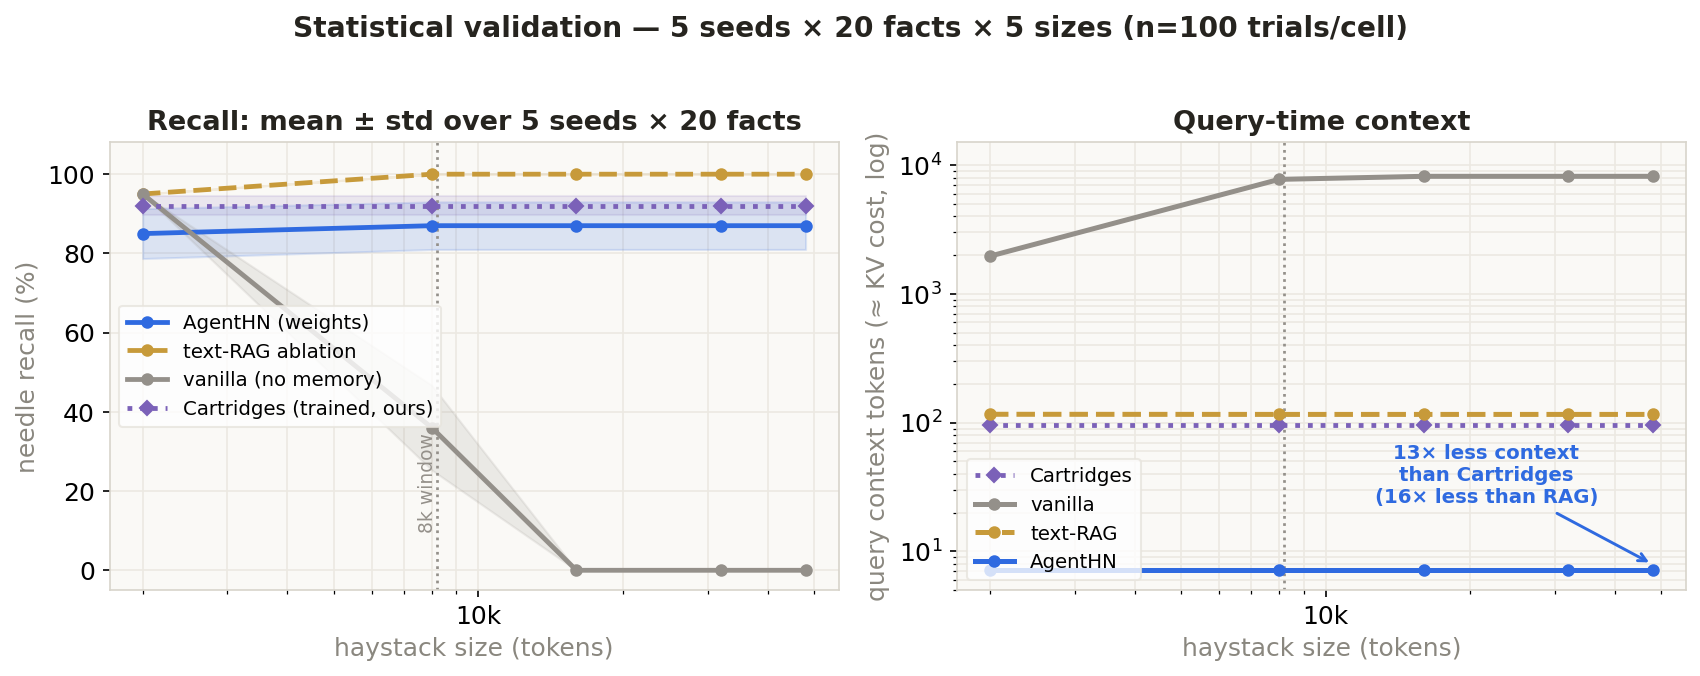
\includegraphics[width=\columnwidth]{figures/large_scale.png}
\caption{Statistical validation: $5$ seeds $\times$ $20$ facts $\times$ $5$ sizes ($n{=}100$/cell), mean $\pm$ std, Wilson 95\% CIs. \mt{scripts/large\_scale\_eval.py}.}
\label{fig:largescale}
\end{figure}

\subsection{Head-to-head against a trained Cartridges baseline}
\label{sec:cartridges}

Cartridges \citep{eyuboglu2025cartridges} trains a small KV-cache prefix \emph{offline}, per corpus, to stand in for that corpus at inference time. We re-implement a faithful, conservative variant -- prefix-tuning \citep{li2021prefixtuning} with $96$ learnable virtual tokens, trained for $60$ epochs per corpus on \emph{paraphrased} question templates (four templates per fact) and evaluated on a fifth, held-out phrasing, so there is no train/test leakage in either direction. This is a lightweight stand-in for Cartridges' full context-distillation self-study pipeline, and we report it as a conservative lower bound on their method's quality, not as a reproduction of their paper's own numbers. Over the same $5$ seeds $\times$ $20$ facts, our reimplementation recalls $92.0\%$ (CI $[85.0,95.9]$) at its fixed $96$-token prefix.

Table~\ref{tab:landscape} places all four methods on one footing. \naplora{} uses $13.3\times$ less query-time context than our Cartridges reimplementation ($7.2$ vs.\ $96$ tokens) and is $1.8\times$ cheaper per query ($0.47$ vs.\ $0.85$ milli-dollars,\footnote{Milli-dollars (m\$) $=10^{-3}$ USD; computed at representative frontier rates of \$3/\$3.75/\$0.30/\$15 per million input/cache-write/cache-read/output tokens (\mt{scripts/cost\_model.py}), for a $48$k-token history queried $1{,}000$ times.} at warm cache), at a cost of $5$ recall points ($87\%$ vs.\ $92\%$). Crucially, Cartridges cannot update mid-conversation -- its $\sim\!43$ (order-of-magnitude estimated) one-time training cost only amortizes over a fixed corpus queried many times, whereas \naplora{}'s creation cost is one hypernetwork forward pass per segment (\$0.14 to encode the entire $48$k-token history), making it the only one of the four methods usable as the conversation is still being written. Figure~\ref{fig:cost} totals these costs over $1{,}000$ queries against a $48$k-token history: vanilla \$14.88 (even with a $10\times$ prefix-cache discount, it still re-reads the full $48$k prefix every query), RAG \$0.84, Cartridges \$44.05 (dominated by the one-time training cost), \naplora{} \$0.61 -- the cheapest of the four.

\begin{table}[t]
\centering\small
\begin{tabular}{lccc}
\toprule
\textbf{Method} & \textbf{Online?} & \textbf{Recall} & \textbf{m\$/query} \\
\midrule
vanilla & yes & 0\% past window & 14.9 \\
RAG & yes & $\sim$100\% & 0.83 \\
Cartridges & \textbf{no} & 92.0\% & 0.85 \\
\naplora{} & yes & 87.0\% & \textbf{0.47} \\
\bottomrule
\end{tabular}
\caption{Method landscape at warm cache, $48$k-token history. Cartridges additionally pays $\sim$\$43 one-time, offline. \mt{scripts/cost\_model.py}.}
\label{tab:landscape}
\end{table}

\begin{figure}[t]
\centering
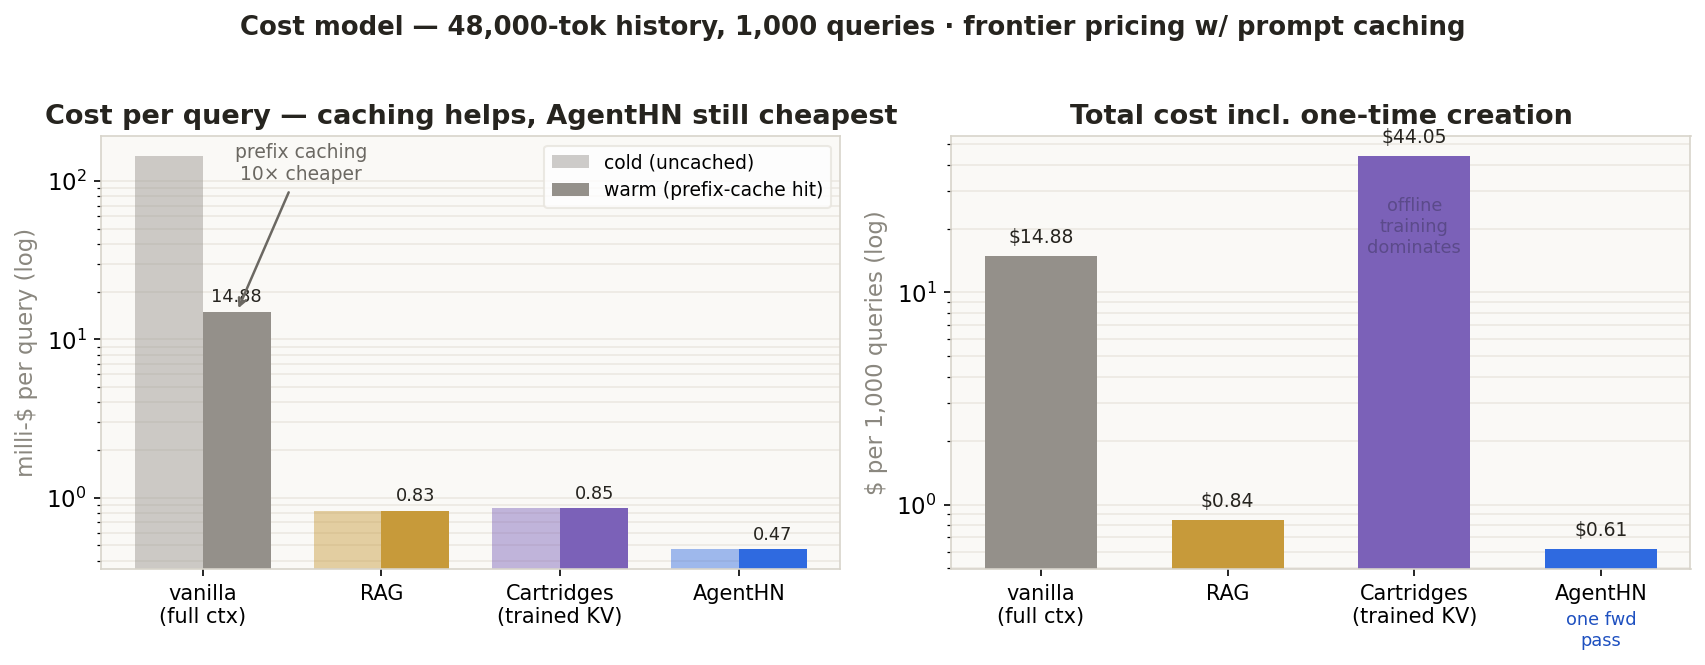
\includegraphics[width=\columnwidth]{figures/cost.png}
\caption{Cost per query and total cost over $1{,}000$ queries against a $48$k-token history, at representative frontier API pricing with prompt caching. \mt{scripts/cost\_model.py}.}
\label{fig:cost}
\end{figure}

\paragraph{Honest framing.} We do not read these numbers as ``\agenthn{} beats Cartridges.'' They optimize different axes: Cartridges is the right tool for a \emph{fixed} corpus queried thousands of times, where offline training amortizes and full self-study distillation likely closes some of the $5$-point recall gap we observe with our conservative reimplementation. \naplora{} is the right tool when the corpus \emph{is} the conversation, still being written, and the memory must update inside the same session that produces it.

% =====================================================================
\section{Personalization}
\label{sec:personalization}
% =====================================================================

The personalization track tests whether \DTL{} internalization generalizes from the static, externally-authored documents it was meta-trained on (encyclopedic QA passages) to a \emph{free-form profile the agent builds about itself, from its own conversation, using no external model or labeled data}. A lightweight extractor prompts the same $2$B base model, after every user turn, to emit zero or more \mt{ACTION | CATEGORY | VALUE} lines (add / update / remove), which are applied to a per-user profile store; an ``I went vegan'' update can retract an earlier ``loves steak'' fact rather than merely contradicting it. The rendered profile doc never enters the prompt -- it exists only to be internalized.

In a representative run, four conversational turns (\emph{``I just moved to Seattle and I work as an ICU nurse,''} \emph{``I'm vegetarian, always hunting for good meatless recipes,''} \emph{``I have a golden retriever named Biscuit who joins me on hikes,''} \emph{``Please keep your answers short and to the point''}) yield seven structured facts (location, profession, dietary preference, a named interest, pet, hobby, communication style). A single \emph{repersonalize} event internalizes the rendered profile doc into one adapter, replacing (not accumulating onto) any prior version, since each user has exactly one current profile. A brand-new session -- empty context, \mt{model.reset()} -- is then asked four held-out questions. With the adapter restored, \emph{``Where do I live?''} $\to$ \emph{``Seattle''} and \emph{``What's my dog's name?''} $\to$ \emph{``Biscuit''}; with the adapter switched off, the identical questions to the identical base model produce \emph{``As an AI, I don't have access to your personal information, including your location''} and the analogous refusal for the dog's name. The only difference between the two columns is whether one cached adapter is bound before generation -- the prompt is byte-for-byte identical and contains zero tokens of profile information either way. This demonstrates persistence across a \emph{session boundary} purely in weight space, a setting \DTL{}'s own evaluations (single document, immediate in-session QA) do not test.

% =====================================================================
\section{Skill Acquisition}
\label{sec:skills}
% =====================================================================

We evaluate reference-document internalization -- giving an agent a ``skill'' once so it need not re-read the skill's documentation on every future use -- across three settings of increasing generality.

\subsection{Formula-sheet acquisition, with statistics}
\label{sec:physics}

Twenty held-out Newton's-laws word problems are answered three ways by the same base model: \textbf{base} (cold, no help), \textbf{in-context} (the full formula-and-worked-examples reference doc pasted into every prompt), and \textbf{adapter} (the doc internalized once via \DTL{}, then \emph{nothing} pasted into the prompt). Grading is numeric-tolerance matching ($2\%$ relative) against the analytically correct answer. Base scores $25\%$ ($5/20$); in-context scores $50\%$ ($10/20$) at an average of $1707.3$ input tokens per question; the adapter scores $55\%$ ($11/20$) at $53.4$ input tokens per question -- a $32\times$ reduction in query-time context that \emph{also} edges out keeping the document in the prompt on accuracy (Figure~\ref{fig:physics}), because internalization is paid once at acquisition time rather than re-paid, identically, on every one of the twenty questions. Internalizing the $\sim\!1.3$k-token doc takes $1.32$ seconds.

\begin{figure}[t]
\centering
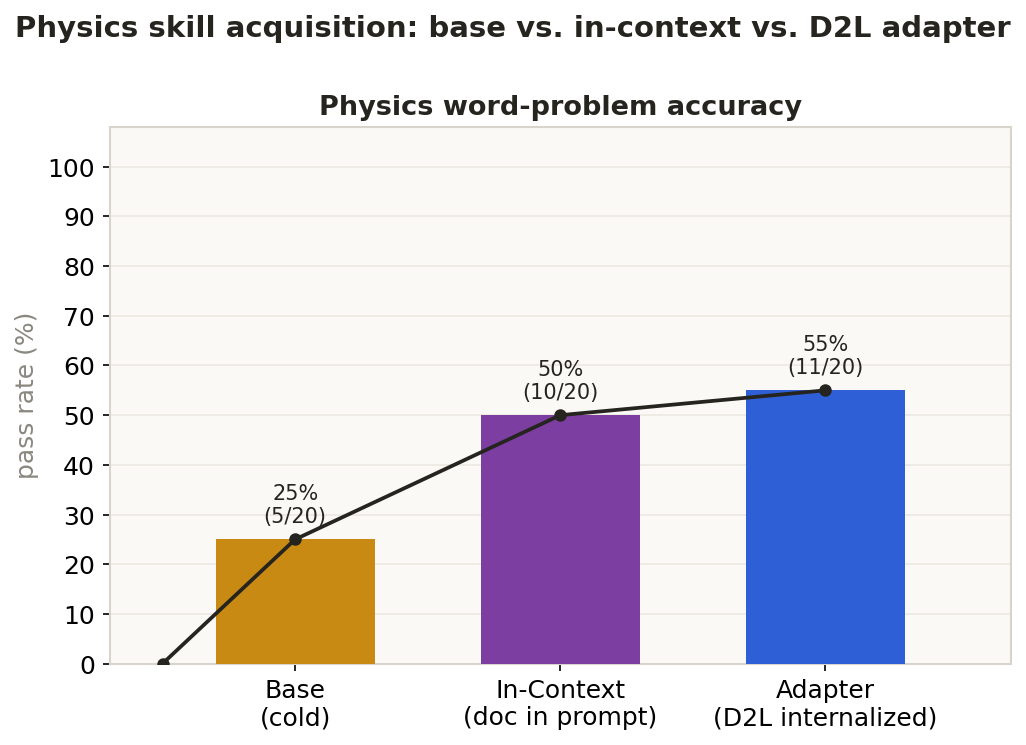
\includegraphics[width=0.48\columnwidth]{figures/accuracy_by_condition.png}
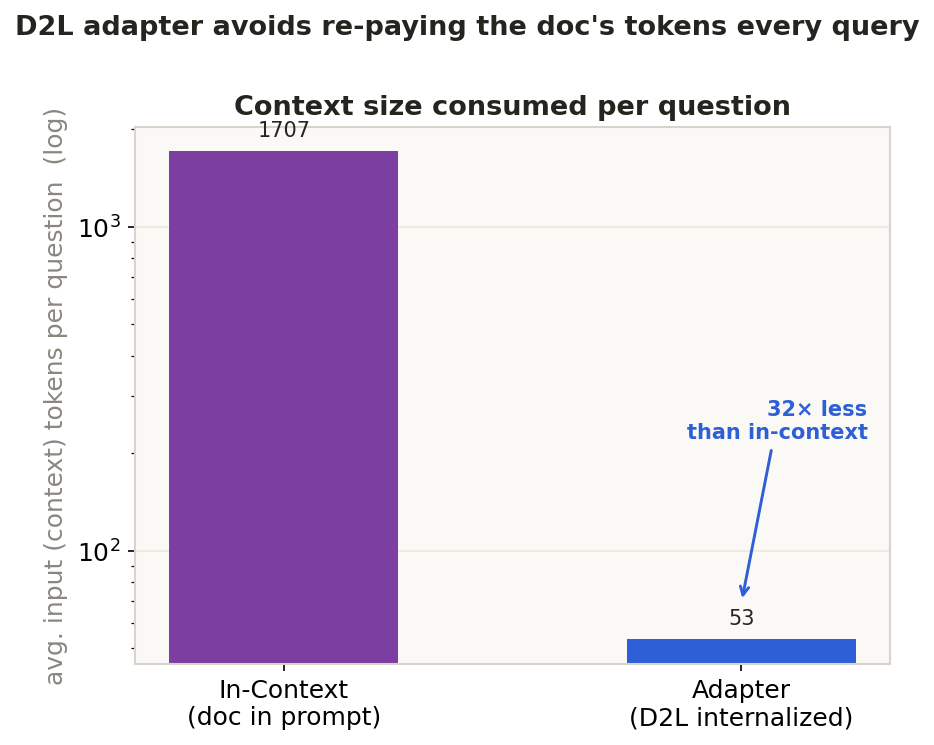
\includegraphics[width=0.48\columnwidth]{figures/context_tokens.png}
\caption{Physics word-problem accuracy (left) and query-time context (right): base vs.\ in-context vs.\ \DTL{} adapter, on $20$ held-out problems. \mt{skill-acquisition/make\_physics\_charts.py}.}
\label{fig:physics}
\end{figure}

\subsection{A skill router, and the need for a behavioral nudge}

A second evaluation tests two skill families behind one classifier: physics word problems and structured-output requests (JSON / YAML / protobuf / bulleted lists), graded by \emph{structural} validity (\mt{json.loads}, \mt{yaml.safe\_load}, a protobuf field regex, a bullet-line regex) rather than exact-match, generalizing the evaluation methodology itself beyond closed-form numeric answers. A bare classification prompt routes an incoming question to \texttt{physics} or \texttt{formatting} (falling back to keyword matching on a classifier parse miss), surfaces that skill's reference doc, internalizes it once (cached per skill thereafter), and re-asks the identical question with the adapter restored and nothing pasted into the prompt.

One engineering finding is worth isolating: \DTL{} internalizes \emph{knowledge}, but not necessarily the \emph{behavioral framing} needed to apply it in the expected style. The physics doc's worked examples all begin ``Let's think step by step.''; without prepending that exact string as an assistant-turn prefill, the internalized model free-styles a verbose, header-and-bullet preamble and clips before reaching the arithmetic under a fixed token budget. A one-line, skill-level, reusable prefill (cost: a handful of tokens, shared across every question that skill answers) is necessary alongside the adapter to reliably invoke the internalized behavior -- internalization supplies the knowledge, a fixed nudge supplies the behavior to use it, and neither alone is enough.

\subsection{Generalizing beyond formula sheets}

A third, smaller experiment internalizes a procedural skill document unrelated to either benchmark: a systematic-debugging skill file (sourced from an open-source agentic-coding skill library\footnote{\url{https://github.com/obra/superpowers}}) whose core principle is ``no fixes without root-cause investigation first.'' Asked for the skill's ``Iron Law'' in one sentence, the base model gives a generic, incorrect answer (\emph{``...break down the problem into smaller, manageable pieces''}); with the doc internalized, the same model correctly states \emph{``...always find the root cause before attempting to fix it.''} Both outputs are verified deterministic under greedy decoding (two independent generations match), and the exported adapter file reproduces the identical output when reloaded from disk without re-internalizing -- adapters are a portable, cacheable artifact, not merely an ephemeral runtime object, and the internalization mechanism generalizes from closed-form, numeric formula sheets to open-ended, principle-based procedural documents.

% =====================================================================
\section{Self-Improvement}
\label{sec:selfimprovement}
% =====================================================================

The self-improvement track asks whether the reflect-and-rewrite loop common to self-refine agents \citep{madaan2023selfrefine,shinn2023reflexion} can operate entirely in weight space: instead of rewriting a chat response, the agent rewrites a LoRA adapter, each round, with no gradient ever computed.

\textbf{Setup.} Sixteen held-out customer-support questions concern a deliberately \emph{fictional} SaaS product (``Lumen''), described in a $347$-token reference document (pricing tiers, refund policy, integrations, feature gating). Grading is accepted-substring matching after normalization, with a placeholder guard that rejects template-shaped answers (e.g.\ \mt{[Plan Name]}) so the model cannot satisfy the grader by echoing a fill-in-the-blank form. \textbf{Round 0} (cold, no doc, no adapter) scores $3/16=18.75\%$ -- not exactly zero, because a $2$B model carries generic priors over plausible SaaS pricing (e.g.\ guessing a Pro tier near \$$29$/month) that occasionally land correctly; the fictional product controls for memorizing \emph{this} company, not for the model's prior over SaaS pricing schemas in general, which we flag as a validity caveat. \textbf{Round 1}: the model studies the reference doc and writes its own $\sim\!5$-sentence notes (not the literal source text), which are internalized into a fresh adapter; retested with nothing but the bare question in the prompt, accuracy rises to $6/16=37.5\%$. \textbf{Round 2}: the model is told only \emph{which} of the sixteen questions it still answered wrong -- no answer key -- and must relocate the relevant facts itself by re-reading the full source document; it rewrites its notes accordingly and re-internalizes: $9/16=56.25\%$, the best round observed. \textbf{Round 3}: the same reflect-rewrite-reinternalize step, once more: $8/16=50.0\%$ -- a dip below round 2.

\begin{figure}[t]
\centering
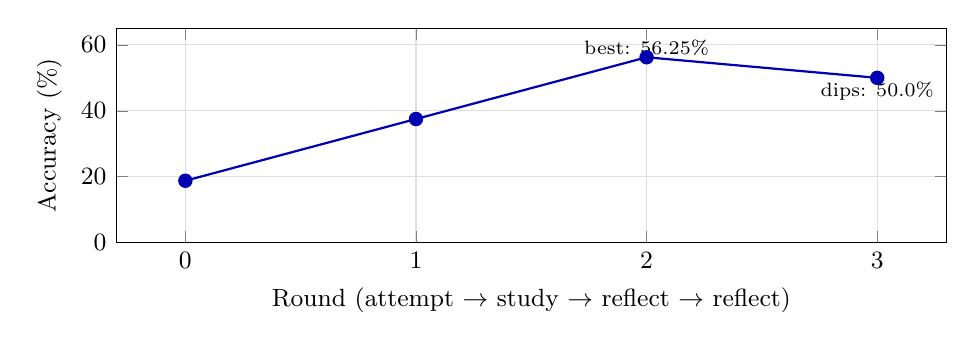
\begin{tikzpicture}
\begin{axis}[
  width=\columnwidth, height=4.3cm,
  xlabel={Round (attempt $\to$ study $\to$ reflect $\to$ reflect)},
  ylabel={Accuracy (\%)},
  xtick={0,1,2,3}, ytick={0,20,40,60},
  ymin=0, ymax=65, xmin=-0.3,xmax=3.3,
  grid=major, grid style={gray!25},
  tick label style={font=\small}, label style={font=\small},
  every axis plot/.append style={thick}
]
\addplot[color=blue!70!black, mark=*, mark size=2.2pt] coordinates {
  (0,18.75) (1,37.5) (2,56.25) (3,50.0)
};
\node[font=\scriptsize] at (axis cs:2,59) {best: 56.25\%};
\node[font=\scriptsize] at (axis cs:3,46) {dips: 50.0\%};
\end{axis}
\end{tikzpicture}
\caption{Self-improvement accuracy trajectory, real numbers, no keep-best ratchet: $18.75\% \to 37.5\% \to 56.25\% \to 50.0\%$. At every round, the test prompt contains only the bare question. \mt{src/agenthn/webapp/skills\_service\_product.py}.}
\label{fig:selfimprove}
\end{figure}

We deliberately report round 3's accuracy as the final number rather than the best-of-rounds ($56.25\%$ at round 2): a hill-climbing loop built from iterative rewriting and re-internalization is not guaranteed to be monotonic, paralleling known non-monotonicity in RL-style and self-refine fine-tuning loops, and reporting the raw trajectory (Figure~\ref{fig:selfimprove}) rather than cherry-picking the best checkpoint is the more defensible practice. The headline result is not the specific numbers but the mechanism: at every single round, the model that is tested has \emph{nothing} in its prompt but the bare question -- everything it has learned so far, including its own self-critique from the previous round, lives in the adapter's weights, and that adapter is replaced, not fine-tuned, every round.

% =====================================================================
\section{Discussion}
% =====================================================================

Across all four tracks, the same primitive -- internalize a document into an adapter in one forward pass, then evict the document from the prompt -- recurs with different documents: an evictable conversation segment (memory), a self-extracted preference profile (personalization), a reference doc or procedural file (skills), and an agent's own self-written, iteratively-revised notes (self-improvement). The one place this primitive needed augmentation rather than direct reuse is memory: \DTL{}'s native chunk-concatenation is built for one bounded document, and applying it na\"ively to an open-ended stream produces destructive interference once enough segments accumulate (\S\ref{sec:interference}). The fix -- retrieve before you compose -- is simple, but the ablation in Table~\ref{tab:ablation} shows it is not optional: every condition that skips it scores $0/6$, regardless of whether the underlying per-segment encoding is in principle capable of perfect recall.

The recurring trade we observe against text-based retrieval is consistent across both memory and skills: a $\sim$two-order-of-magnitude reduction in query-time context, in exchange for $5$--$13$ points of recall, because the hypernetwork's encoding is lossy in a way that exact text retrieval is not. Whether that trade is worth it is a deployment decision, not a universal answer -- it is attractive exactly when query-time context cost (latency, KV-cache memory, dollars) dominates the cost of being occasionally wrong, and a $2$B base model's residual encoding capacity is the binding constraint on how small that ``occasionally'' can be made; we would expect the recall side of this trade to improve with a larger base model and a hypernetwork trained at matching scale, since \DTL{}'s own architecture does not depend on model size.

% =====================================================================
\section*{Limitations}
% =====================================================================

\paragraph{Single small base model.} Every result in this paper uses one $2$B-parameter base model (\mt{gemma-2-2b-it}) and one released \DTL{} checkpoint. The $2$B model's limited residual capacity is almost certainly the dominant source of the lossy-recall gap we observe (e.g.\ ``Ayemi'' vs.\ ``Adeyemi,'' \S\ref{sec:memory}), and our skill-acquisition ceiling ($55\%$ on physics word problems) reflects the base model's reasoning ability as much as the internalization mechanism. We have not evaluated whether our findings -- particularly the destructive-interference failure mode and the retrieval fix -- hold at larger scale.

\paragraph{Lossy compaction is fundamental, not incidental.} \naplora{} consistently trades recall for context cost relative to retrieving text; we report this honestly (\S\ref{sec:largescale}, \S\ref{sec:cartridges}) rather than presenting only favorable comparisons, but the gap means \naplora{} is not a drop-in replacement for RAG wherever recall is the only thing that matters.

\paragraph{Estimated costs.} Our Cartridges training-cost estimate (\S\ref{sec:cartridges}, $\sim$\$43 per corpus) is an explicitly order-of-magnitude, labeled estimate (modeled as $300\times$ the cost of one read of the corpus), not a directly measured wall-clock training bill; our Cartridges \emph{recall} number, by contrast, is measured from an actual trained model and should not be conflated with the cost estimate's precision.

\paragraph{Synthetic evaluation.} Our memory and self-improvement probes use synthetic, deliberately unguessable facts and a fictional product specifically so that no result can be attributed to the base model's pretraining priors about a real entity. This is the right design for isolating the mechanism, but it limits ecological validity relative to real, messy long-horizon agent transcripts, which we have not evaluated on.

\paragraph{Non-monotonic self-improvement.} The self-improvement trajectory (\S\ref{sec:selfimprovement}) dips at round 3; we have no mechanism that guarantees monotonic improvement, and a practitioner deploying this loop would need an external stopping criterion (e.g.\ a held-out validation slice) rather than assuming more rounds are always better.

\paragraph{Checkpoint-specific multi-chunk support.} The publicly released \DTL{} checkpoints differ in whether multi-chunk rank-concatenation is in-distribution; using the single-chunk-trained checkpoint for memory composition silently produces degenerate adapters rather than raising an error, a sharp edge we encountered directly during development and flag for anyone reproducing this work.

% =====================================================================
\section*{Ethical Considerations}
% =====================================================================
The personalization track stores user-specific preferences in model weights rather than in a plaintext profile, which could plausibly be read as more private (the profile text never sits in a server log of prompts) or less private (a weight delta is non-human-readable but not necessarily harder to extract via probing); we have not evaluated extraction attacks against internalized adapters and recommend treating an adapter as containing the same sensitive information as the document it was built from. All synthetic facts, the fictional ``Lumen'' product, and the held-out physics/formatting questions in this paper are fabricated for evaluation purposes and do not reference real individuals, companies, or proprietary material.

% =====================================================================
\section{Conclusion}
% =====================================================================

We presented \agenthn{}, a framework for letting agents edit their own weights at inference time via the Doc-to-LoRA hypernetwork, and \naplora{}, a streaming memory mechanism that extends \DTL{}'s bounded single-document chunking into an unbounded conversational horizon by adding retrieval-gated composition -- without which the natural extension fails completely via destructive interference. Across memory, personalization, skill acquisition, and self-improvement, internalizing a document into an adapter and evicting it from the prompt consistently trades a measurable, bounded amount of recall for an order-of-magnitude reduction in query-time context and cost, with no gradient training at inference time in any of the four tracks. We release all code, evaluation scripts, captured fixtures, and the exact numbers reported in every table and figure of this paper.

\section*{Acknowledgments}
We thank Sakana AI for releasing Doc-to-LoRA's code and checkpoints, without which none of this work would have been possible, and the organizers of the hackathon this project began at.

% =====================================================================
\bibliographystyle{acl_natbib}
\bibliography{references}

% =====================================================================
\appendix

\section{Prompts}
\label{app:prompts}

\paragraph{Personalization extractor (\S\ref{sec:personalization}).} The base model is prompted, after every user turn, with a fixed instruction to output zero or more lines of the form \mt{ACTION | CATEGORY | VALUE} (\mt{add}/\mt{update}/\mt{remove}; \mt{NONE} if nothing durable is said), with two worked examples (a moving/profession update, a dietary-preference correction) included in the prompt to anchor the line format, since a $2$B model is unreliable at emitting well-formed JSON for this task.

\paragraph{Self-improvement study/reflect prompts (\S\ref{sec:selfimprovement}).} Round 1: \emph{``Read the following product reference material and write concise study notes (about 5 sentences) capturing the most important facts a support agent would need.''} Later rounds: the model is shown its current notes and the list of \emph{questions} (not answers) it got wrong, and instructed to \emph{``find the facts these questions ask about in the reference material and rewrite your study notes so you can answer them next time,''} explicitly keeping whatever in the old notes remains useful rather than discarding it.

\paragraph{Skill-router classifier (\S\ref{sec:skills}).} \emph{``Classify the question below into exactly one category: PHYSICS (a mechanics word problem...) or FORMATTING (a request to produce structured output like JSON, YAML, protobuf, or a bulleted list). Reply with one word.''}

\section{Full statistical validation table}
\label{app:largescale}

\begin{table}[h]
\centering\small
\begin{tabular}{rrrr}
\toprule
\textbf{Size} & \textbf{\naplora{}} & \textbf{text-RAG} & \textbf{vanilla} \\
\midrule
2k  & 85.0 (7.2) & 95.0 (116.1) & 95.0 (1964.0) \\
8k  & 87.0 (7.2) & 100.0 (115.8) & 36.0 (7755.8) \\
16k & 87.0 (7.2) & 100.0 (115.8) & 0.0 (8192.0) \\
32k & 87.0 (7.2) & 100.0 (115.8) & 0.0 (8192.0) \\
48k & 87.0 (7.2) & 100.0 (115.8) & 0.0 (8192.0) \\
\bottomrule
\end{tabular}
\caption{Pooled recall \% (query-time context tokens), $n{=}100$ trials/cell ($5$ seeds $\times$ $20$ facts). \mt{results/large\_scale.json}.}
\end{table}

\section{Scaling sweep, full table}
\label{app:scaling}

\begin{table}[h]
\centering\small
\begin{tabular}{rrrrr}
\toprule
\textbf{Target} & \textbf{Raw tok} & \textbf{Segs} & \textbf{\naplora{}} & \textbf{Vanilla} \\
\midrule
1k  & 1{,}025  & 10  & 6/6 & 6/6 \\
2k  & 2{,}029  & 19  & 6/6 & 6/6 \\
4k  & 4{,}004  & 36  & 6/6 & 6/6 \\
8k  & 8{,}002  & 70  & 6/6 & 4/6 \\
16k & 16{,}009 & 138 & 6/6 & 0/6 \\
32k & 32{,}023 & 274 & 6/6 & 0/6 \\
48k & 48{,}006 & 410 & 6/6 & 0/6 \\
\bottomrule
\end{tabular}
\caption{Six-needle recall as one conversation grows to $48$k tokens. \naplora{}'s query-time context stays at $9.5$ tokens throughout (vs.\ vanilla growing to the $8{,}192$-token window cap). \mt{scripts/scaling\_sweep.py}.}
\end{table}

\section{Held-out physics word problems}
\label{app:physics}
Representative items from the $20$-question battery (\S\ref{sec:physics}; full list in \mt{skill-acquisition/golden-examples.txt}): \emph{``A 15 kg box sits on a horizontal floor with a coefficient of friction of 0.3. What is the maximum friction force?''} (expected $44.1$N); \emph{``Two masses of 10 kg and 3 kg are 2 m apart. What is the gravitational force between them ($G=6.674\times10^{-11}\,\mathrm{N\,m^2/kg^2}$)?''} (expected $5.0055\times10^{-10}$N); \emph{``A 1000 kg car accelerates from rest to 20 m/s in 4 seconds. What net force acted on the car?''} (expected $5000$N).

\section{Reproducibility}
\label{app:repro}
All numbers in this paper are produced by scripts committed in the project repository and read programmatically from their JSON outputs (\mt{results/*.json}, \mt{skill-acquisition/physics\_benchmark\_results.json}) rather than transcribed from figures. Base model: \mt{google/gemma-2-2b-it} (gated) / \mt{unsloth/gemma-2-2b-it} (ungated mirror, identical weights) throughout. Greedy decoding (\mt{do\_sample=False}) is used for every numeric result reported; sampling temperature is not a free parameter anywhere in this paper.

\end{document}
